\chapter{Estado da arte}



Nesta secção, são apresentados os resultados da pesquisa efectuada sobre o
estado da arte das ferramentas com funcionalidades que deverão estar presentes no sistema desenvolvido. Pretende-se apresentar de forma geral todas as tecnologias possíveis de utilização e respetiva comparação. 


\section{\acl{SGBD}}

Um \ac{SGBD} é um conjunto de software responsáveis pela gestão de uma base de dados.






\subsection{MySQL}



\subsection{SQL server}



\subsection{PostgreSQL}

O PostgreSQL é um sistema de gestão de base de dados do tipo objeto-relacional uma vez que permite um modelo de dados orientado a objetos, isto é, possibilita a manipulação de objetos, classes e heranças diretamente no esquemas da base de dados. Segundo o site oficial do PostgreSQL este é considerado um \ac{SGBD} bastante poderoso e com desenvolvimento \textit{open sources} \cite{ThePostgreSQLGlobalDevelopmentGroup2012}. 


%Ele tem mais de 15 anos de desenvolvimento ativo e uma arquitetura comprovada que ela ganhou uma forte reputação de confiabilidade, integridade de dados e correção. Ele roda em todos os principais sistemas operacionais, incluindo Linux, UNIX (AIX, BSD, HP-UX, SGI IRIX, MacOS, Solaris, Tru64), e Windows. É totalmente compatível com ACID, tem suporte completo para chaves estrangeiras, junções views, triggers e procedimentos armazenados (em várias línguas). Ele inclui mais SQL: 2008 tipos de dados, incluindo INTEGER, NUMERIC, BOOLEAN, CHAR, VARCHAR, DATE, INTERVALO e TIMESTAMP. Ele também suporta o armazenamento de grandes objetos binários, incluindo imagens, sons ou vídeo. Ele tem interfaces de programação nativas para C / C ++, Java, .Net, Perl, Python, Ruby, Tcl, ODBC, entre outros, e documentação



\subsection{Comparação e solução adotada}


Os próprios criadores do Django recomendam a utilização do PostgreSQL, indicando que alcança um bom equilibrio entre custo, caracterıas, rapidez e estabilidade




No entanto, é pertinente fazer uma comparação entre o PostgreSQL e
outras ferramentas open-source como o MySQL. Embora as diferenças entre
as duas ferramentas não sejam muito grandes, podemos ter também em conta
a performance de uma e outra. Uma comparação feita usando o benchmark
TPC-H 8 mostra que a performance do PostgreSQL é ligeiramente superior à
do MySQL na maioria das queries [22].



\newpage
\section{Desenvolvimento web}



Para o desenvolvimento da dashboard poderiam ser adotadas duas estratégias distintas para o desenvolvimento web: 


A criacao de sites dinamicos que se apdatam ao cliente podem ser alcançados de dois modos: 

\begin{itemize}
	\item Manipulação local usando javascript do DOM. 
	
	\item Acesso ao servidor que serve conteúdos criados em função dos pedidos do cliente
	
\end{itemize}



Neste contexto poderiam ser utilizados 


Angular, React

Servidor serve conteudos criados em função dos pedidos do cliente 







\subsection{ASP.net}

\subsection{Flask}

\subsection{Django}


Assim, e de acordo com as explicações dos autores da ferramenta [18], as
principais vantagens tiradas da utilização da framework Django são:
Boa documentação;
Facilidade e rapidez de desenvolvimento e deployment;
Estabilidade;
Escalabilidade.


\subsection{Conclusões e solução adotada}



\newpage
\section{Desenvolvimento mobile}


http://bloomidea.com/blog/aplicacoes-nativas-vs-hibridas-qual-escolher-para-o-seu-projeto	

\subsection{Plataformas nativas}


uma aplicação móvel nativa é uma app que foi desenvolvida para ser utilizada numa plataforma ou dispositivo específico (iOS ou Android), usando as ferramentas e a linguagem de desenvolvimento correspondentes àquelas que o sistema em questão suporta. Uma app nativa pode assim interagir e tirar partido das funcionalidades do próprio sistema operativo e de outro software que esteja instalado nessa plataforma, o que faz desta opção uma excelente aposta.


\begin{itemize}
	\item \textbf{Performance}: 
	\item \textbf{Desenvolvimento}: 
	\item \textbf{Manutenção}: 
	\item \textbf{Interface}: 
	\item \textbf{Recursos disponíveis}: 
	\item \textbf{\textit{Plug-ins}}: 
	\item \textbf{Segurança}: 
\end{itemize}



\subsection{Multi-plataforma}

http://websocialdev.com/lista-de-frameworks-para-desenvolvimento-mobile/


\begin{itemize}
	\item \textbf{Performance}: 
	\item \textbf{Desenvolvimento}: 
	\item \textbf{Manutenção}: 
	\item \textbf{Interface}: 
	\item \textbf{Recursos disponíveis}: 
	\item \textbf{\textit{Plug-ins}}: 
	\item \textbf{Segurança}: 
\end{itemize}




\subsection{Conclusões e solução adotada}





\newpage
\section{REST Frameworks}




\subsection{Django Rest Framework}





Django REST Framework é uma ferramenta considerada 'poderosa e flexível para a construção de APIs Web' [], que pode ser usada juntamente com a framework de desenvolvimento de aplicações Web Django, que quando integrada no desenvolvimento de um determinado \textit{backend} permite a implementação de serviços do tipo REST.



A API navegável Web é uma vitória usabilidade enorme para os desenvolvedores.

Políticas de autenticação , incluindo pacotes para OAuth1a e OAuth2 .

Serialização que suporta tanto ORM e não ORM fontes de dados.

Customizável todo o caminho - basta usar vistas regulares baseadas na função , se você não  precisar dos mais poderosos recursos .

Extensa documentação , e grande apoio da comunidade .

Utilizado e confiável por empresas internacionalmente reconhecidas, incluindo Mozilla , 
Red Hat , Heroku , e Eventbrite .




\subsection{Flask-RESTful}


\subsection{Restlet}



\subsection{Conclusões e solução adotada}




com autenticação via token 







app mobile
microcontroladores -> controller modulers 


documentação com swager 





\newpage
\section{Micro-controladores}



\subsection{Arduino}


O Arduino é fruto da evolução de um projeto italiano desenvolvido no ano de 2005, cujo o objetivo foi ser utilizado em projetos escolares de forma a ter um orçamento menor que outros sistemas de prototipagem disponíveis naquela época.

Tal como descrito no seu site oficial, um Arduino consiste numa plataforma \textit{open-source} de prototipagem eletrónica com \textit{hardware} e \textit{software} flexíveis e com elevada facilidade utilização[]. O Arduino é utilizado para projetos especialmente no contexto do \ac{IoT} e da robótica educativa. A este micro-controlador, podem ser estendidos vários módulos, dependendo da tarefa que se quer que seja executada. 


O Arduino possui um conjunto de pinos que podem ser programados para funcionarem como entradas ou saídas fazendo com que o Arduino interaja com o meio externo para os mais diversos fins. Para além dos pinos de I/O exitem pinos de alimentação que fornecem diversos valores de tensão que podem ser utilizados para transmitir energia elétrica aos diferentes componentes de um projeto. 

A versão Nano do Arduino, 

Na figura \ref{ard2} e \ref{ard1} apresenta-se uma imagem do arduino utilizado e a identificação dos diferentes pinos existentes, respectivamente. Na tabela \ref{caraarduino} encontram-se as principais características desta versão do Arduino. 


\begin{figure}[h]
	\centering
	\begin{minipage}[b]{0.5\textwidth}
		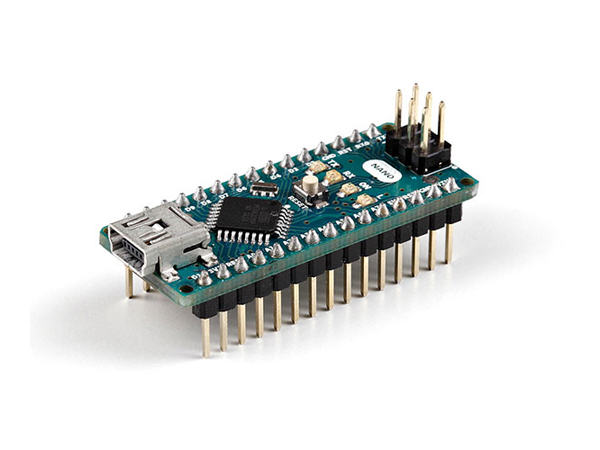
\includegraphics[width=\textwidth]{img/hardware/nano-img.jpg}
		\caption{Arduin Nano}
		\label{ard2}
	\end{minipage}
	\hfill
	\begin{minipage}[b]{0.3\textwidth}
		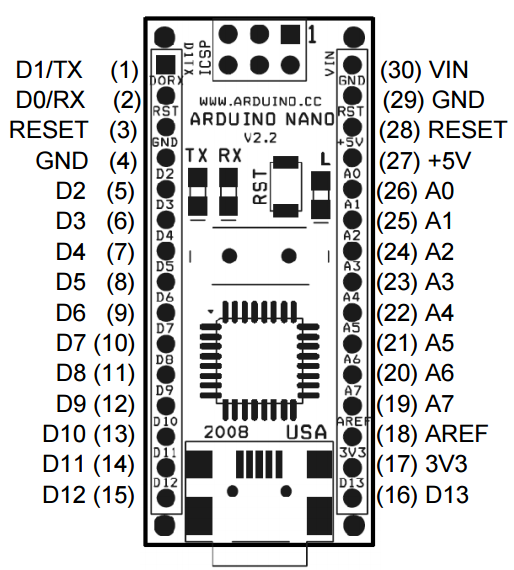
\includegraphics[width=\textwidth]{img/hardware/nano-esquema.png}
		\caption{Identificação dos pinos no Arduino Nano}
		\label{ard1}
	\end{minipage}
\end{figure}








\newpage

\begin{table}[h]
	\centering
	
	\begin{tabular}{|
			>{\columncolor[HTML]{C0C0C0}}l |l|} \hline
		Microcontrolador & ATmega328 \\ \hline
		Tensão de operação & 5V \\ \hline
		Tensão de entrada & 7-12V \\ \hline
		Portas digitais & 14 (6 podem ser usadas como PWM) \\ \hline
		Portas analógicas & 8 \\ \hline
		Corrente nos pinos \ac{I/O} & 40mA \\ \hline
		Memória Flash & 32KB (2KB usado no bootloader) \\ \hline
		Memória \acs{RAM} (SRAM) & 2KB \\ \hline
		EEPROM & 1KB \\ \hline
		Velocidade do Clock & 16MHz \\ \hline
		Dimensões & 45 x 18mm \\ \hline
		LED interno & Pino digital 13 \\ \hline
		Ligação USB & Ligação ao computador e alimentação \\ \hline
	\end{tabular}
	\caption{Características do Arduino Nano}
	\label{caraarduino}
\end{table}






\subsection{Raspberry Pi }

O Raspberry Pi (figura \ref{rasp1}) é considerado um micro-computador do tamanho de um cartão de crédito que possui um conjunto de \textit{hardware} integrado que tal como Arduino possibilita uma interação com o meio exterior. O principal objetivo deste poderoso componente consistiu em promover o ensino da ciência da computação em escolas de ensino básico. 
O Raspberry Pi foi desenvolvido no Reino Unido pela \textit{Raspberry Pi Foundation}.



\newpage
\begin{figure}[h]
	\centering
	\begin{minipage}[b]{0.4\textwidth}
		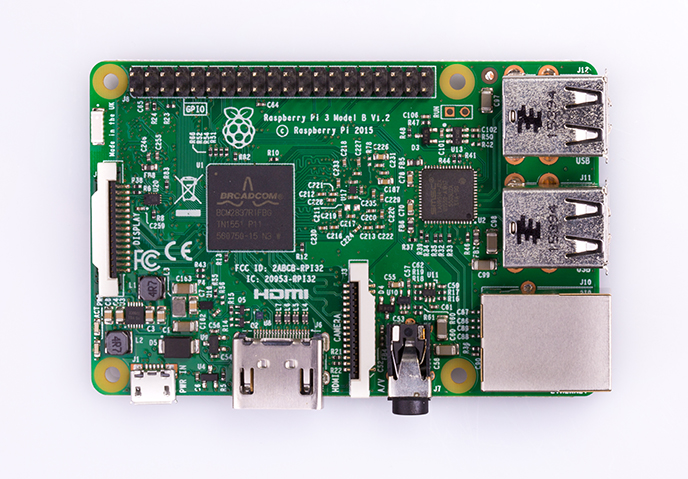
\includegraphics[width=\textwidth]{img/hardware/rasp3-img.jpg}
		\caption{Raspberry Pi 3}
		\label{rasp1}
	\end{minipage}
	\hfill
	\begin{minipage}[b]{0.5\textwidth}
		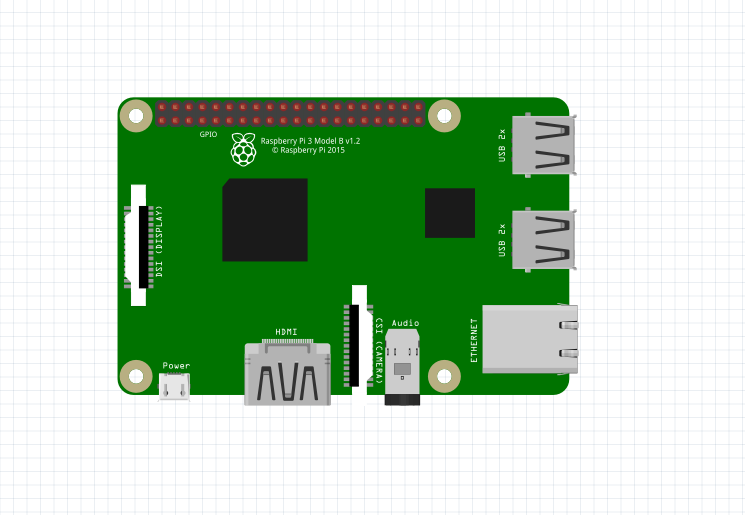
\includegraphics[width=\textwidth]{img/hardware/rasp-esquema.PNG}
		\caption{Identificação dos principais componentes no Raspberry Pi 3 }
	\end{minipage}
\end{figure}




\begin{table}[h]
	\centering
	
	\begin{tabular}{|
			>{\columncolor[HTML]{C0C0C0}}l |l|l|}
		\hline
		& \cellcolor[HTML]{C0C0C0}\textbf{Raspberry Pi 3 Model B} & \cellcolor[HTML]{C0C0C0}\textbf{Raspberry Pi 2 Model B 1.2} \\ \hline
		\textbf{Processor Chipset} & \begin{tabular}[c]{@{}l@{}}Broadcom BCM2837\\ 64Bit  Quad Core \\ Processor powered \\ Single Board Computer\\ running at 1.2GHz\end{tabular} & \begin{tabular}[c]{@{}l@{}}Broadcom BCM2837 64Bit \\ Quad Core Processor \\ powered Single Board \\ Computer running at \\ 900MHz\end{tabular} \\ \hline
		\textbf{Processor Speed} & QUAD Core @1.2 GHz & QUAD Core @900 MHz \\ \hline
		\textbf{RAM} & 1GB SDRAM @ 400 MHz & 1GB SDRAM @ 400 MHz \\ \hline
		\textbf{Storage} & MicroSD & MicroSD \\ \hline
		\textbf{USB 2.0} & 4x USB Ports & 4x USB Ports \\ \hline
		\textbf{\begin{tabular}[c]{@{}l@{}}Max Power \\ Draw/voltage\end{tabular}} & 2.5A @ 5V & 1.8A @ 5V \\ \hline
		\textbf{GPIO} & 40 pin & 40 pin \\ \hline
		\textbf{Ethernet Port} & Yes & Yes \\ \hline
		\textbf{WiFi} & Built  in (802.11n) & No \\ \hline
		\textbf{Bluetooth LE} & Built in (4.1) & No \\ \hline
	\end{tabular}
	\caption{Comparação entre versão 2 e 3 do Raspberry Pi}
	\label{my-label}
\end{table}









\newpage
\section{Sensores}


Esta secção tem como objetivo fazer um estudo comparativo entre diferentes tecnologias usadas para a medição dos vários parâmetros ambientais necessários ao controlo e monitorização da salicornia. Todas as soluções adaptadas tem termos de hardware escolhidas devido à possui-las. 



\subsection{Sensor de salinidade}


\subsection{Sensor de temperatura }
Existem vários tipos de sensores de temperatura baseados em princípios de funcionamento distintos. 


\begin{itemize}
	\item \textbf{Termopares}: 
	\item \textbf{RTDs}:
	\item \textbf{Termístor}: 
	\item \textbf{Circuito integrado}: 
\end{itemize}








\newpage

\subsection{Sensor de luminosidade }


O LDR (Light Dependent Resistor) é um componente cuja resistência varia de acordo com a intensidade da luz. Quanto mais luz incidir sobre o componente, menor a resistência. Este sensor de luminosidade pode ser utilizado em projetos com arduino e outros microcontroladores para alarmes, automação residencial, sensores de presença e etc.





\newpage
\section{Tecnologias de comunicação}

Nesta secção serão apresentados alguns das tecnologias de comunicação mais utilizados em \textit{Internet of Things} que permite a troca de informações entre dispositivos e respetiva comparação entre eles. 




\subsection{Zigbee}

Zigbee designa um conjunto de especificações para a comunicação sem-fio entre dispositivos eletrônicos, com ênfase na baixa potência de operação, na baixa taxa de transmissão de dados e no baixo custo de implementação. Tal conjunto de especificações define camadas do modelo OSI subsequentes àquelas estabelecidas pelo padrão IEEE 802.15.4.


\subsection{LoRa}

A tecnologia Lora

Wide-Area Network Low-Power ( LPWAN ) ou Low-Power Rede ( LPN ) é um tipo de telecomunicações sem fio de rede projetada para permitir comunicações de longo alcance em uma baixa taxa de bits entre as coisas (objetos relacionados), tais como sensores operados em uma bateria.

As tecnologias WAN de baixa potência são projetadas para ambientes de rede máquina a máquina (M2M). Com a diminuição dos requisitos de energia, maior alcance e menor custo do que uma rede móvel, os LPWANs são pensados para permitir uma gama muito mais ampla de aplicativos M2M e Internet of Things (IoT), que foram limitados por orçamentos e problemas de energia.



\subsection{Sigfox}

Uma empresa francesa que constrói redes sem fio para conectar objetos de baixa energia, como medidores de energia elétrica , smartwatches e máquinas de lavar, que precisam estar continuamente ligados e emitindo pequenas quantidades de dados. Sua tecnologia é voltada para a Internet das Coisas (IoT).



\subsection{Bluetooth}

Bluetooth é uma especificação de rede sem fio de âmbito pessoal (Wireless personal area networks – PANs) consideradas do tipo PAN ou mesmo WPAN


\subsection{WiFi}

rede sem fio IEEE 802.11, que também são conhecidas como redes Wi-Fi ou wireless, foram uma das grandes novidades tecnológicas dos últimos anos. Atuando na camada física, o 802.11 define uma série de padrões de transmissão e codificação para comunicações sem fio, sendo os mais comuns: FHSS (Frequency Hopping Spread Spectrun), DSSS (Direct Sequence Spread Spectrum) e OFDM (Orthogonal Frequency Division Multiplexing). Atualmente, é o padrão de fato em conectividade sem fio para redes locais. Como prova desse sucesso pode-se citar o crescente número de Hot Spots e o fato de a maioria dos computadores portáteis novos já saírem de fábrica equipados com interfaces IEEE 802.25. A Rede IEEE possui como principal característica transmitir sinal sem fio através de ondas!




\subsection{Comparação de tecnologias de comunicação}





%\subsection{Módulo bluetooth}







\newpage
\section{Aplicações relacionadas}



Seja para comparar, seja para replicar boas funcionalidades, ou seja para conseguir oferecer algo mais ao utilizador final, quando se pretende desenvolver uma determinada aplicação, e
importante proceder a uma avaliação de aplicações da mesma área se encontram no mercado.
Assim, são aqui abordadas algumas das aplicações relacionadas que são mais utilizadas ou que mais se aproximam daquilo que se pretende para a aplicação a desenvolver neste projeto,
tendo em conta os diferentes sistemas operativos.



\subsection{Multi-monitorização de estufas agrícolas }

https://repositorio.ipcb.pt/bitstream/10400.11/949/1/Multimonitorizacao%20Estufa%20Agricola.PDF

\subsection{Agroopar}

http://www.vidarural.pt/agroopar-os-custos-na-mao-do-agricultor/


\subsection{outras que vale a pena para comparacao..}

%\subsection{Sistema de Monitorização de Estufas Agrícolas}


\cite{Abreu2012}


\newpage









